\subsection{Middlewares} 
Um middleware comporta-se como uma ligação entre porções de código, sendo possível este também executar código.

\subsubsection{Linguagem}
O bem essencial em uma boa comunicação entre duas partes é a utilização da mesma linguagem, sendo assim foi necessário perceber qual a linguagem a utilizar quando se responde a um pedido. Para este fim foi então desenvolvido um middleware, o objetivo deste é verificar se existe a chave language no cabeçalho do pedido, caso esta exista é então obtido a linguagem e guardada nas variáveis locais do pedido. Em caso de esta tag não existir, foi então decidido que a aplicação responderá em português por omissão, este valor poderá ser futuramente alterado de forma simples.

\newpage

\subsubsection{Autenticação}
De forma a assegurar a autenticação dos utilizadores que necessitam desta foi então decidido implementar JsonWebToken, este tipo de autenticação baseia-se em a utilização de tokens com tempo de expiração, sendo que enquando o token estiver válido, o utilizador poderá realizar pedidos e assim que este token expirar este terá de se autenticar novamente para obter um novo token.
A utilização de tokens permite também assegurar que os pedidos são realizados com tokens gerados pela api através de utilização de uma chave de assinatura de token, impedindo assim a utilização de tokens gerados por utilizadores.
\begin{figure}[htb]
  \centering
  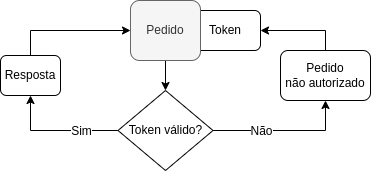
\includegraphics[width=0.5\textwidth]{images/implementacao/api/jwt_session.png}
  \caption{Exemplo de página de produto incomum}
  \label{fig:64}
\end{figure}

A grande valia da utilização a técnica de autenticação mencionada anteriormente é a segurança desta, mas este nivel de segurança leva a que as aplicações que não necessitam de um nivel de segurança muito alto se tornem impráticas. Isto acontece porque estes  tokens têm geralmente uma duração muito curta como por exemplo 15 minutos, e sempre que um token de sessão expira o utilizador 
teria de realizar novamente o login.

A solução deste problema sem a perda de segurança significativa veio pelo meio da utilização de tokens de duração maior em conjunto com os tokens de duração curta, sendo que enquanto o token de grande duração estiver válido, novos tokens de curta duração são gerados para o utilizador nunca perdendo assim a sua sessão. Estes tokens de grande duração tem por nome tokens de refresh e os tokens de curta duração têm por nome tokens de sessão. Sempre que o utilizador termina a sua sessão o token de refresh deverá ser apagado.

Sempre que um utilizador realiza um pedido o seu token de sessão deverá ser validado, caso este seja válido, o seu token de refresh deverá também ser validado e apenas após isto o utilizador estará autenticado. Caso o token de sessão ou de refresh esteja expirado, este continuará a estar sem autorização para realizar o pedido, mas poderá pedir um novo token de sessão enquanto o seu token de refresh estiver válido, isto acontece sem realizar novamente o login e sem o utilizador perceber.

 Além das funcionalidades atrás mencionadas é possível também associar dados em formato json a um token jwt, esta funcionalidade foi utilizada para enviar o id do utilizador a qual pertence este token e também o cargo do mesmo.

 \newpage

\subsubsection{Validação de Papel}

Com finalidade de garantir que apenas empresas podem realizar os pedidos de empresas e apenas técnicos e empresas podem realizar os pedidos de técnicos foi então criado um middleware que valida se o utilizador que realizou o pedido tem permissões para o mesmo. Este middleware interliga-se com o middleware anterior pois como mencionado o cargo do utilizador em questão é enviado no token, sendo assim é obtido este cargo e realizada uma comparação, com o cargo desejado. Para isto foram criados 2 middlewares diferentes, um valida o cargo de empresas e o outro o cargo de técnicos. Visto que as empresas podem realizar operações de técnicos então no middleware de técnicos é verificado se o token corresponde a um utilizador empresa ou a um utilizador técnico, já no middleware de validação de empresa é verificado se o utilizador tem cargo de empresa.


%TODO: Adicionar esquema a mostrar como estes middlewares funcionam
